\documentclass[a4paper,11pt]{article}%,twocolumn
\input{settings/packages}
%% page settings
\usepackage[top=10mm, bottom=15mm,left=10mm,right=10mm]{geometry}  
 % needed for page border settings
\parindent=0mm % for space of first line of new text block

\sloppy % for writing with hyphenless justification (tries to)
\hyphenation{} % use hyphenation of tolerance parametershttp://www.jr-x.de/publikationen/latex/tipps/zeilenumbruch.html
\hyphenpenalty=10000
\exhyphenpenalty=10000
\usepackage{fancyhdr} % needed for head and foot options
\input{settings/jupyter}
\usepackage{fontawesome}

\begin{document}
	\begin{center}
	{\large \textbf{Assignment A04: Neural Networks}}\\
	Thalagala B.P.\hspace{0.5cm} 180631J 
\end{center}
\hrule


\hspace{10mm}


\textit{\textbf{Data set:} CIFAR10 50,000 32$\times$32$\times$3 training images and 10 classes. Accuracy greater than 0.1 shows learning.}
\section*{Part 1}

For the linear classifier in {\tt cell 2}, the score function is $f(x) = Wx +b$. But Keeping track of two sets of parameters \textbf{\textit{W}} and \textit{\textbf{b}} separately is not really efficient in computation. This cumbersomeness can be eliminated by combining both of them into one single matrix as coded in {\tt cell 1}. Additionally a column of ones must be added in front of training and testing images matrices({\tt x\_train,x\_test}) to enable matrix multiplication after this rearrangement.\\

    \begin{tcolorbox}[breakable, size=fbox, boxrule=1pt, pad at break*=1mm,colback=cellbackground, colframe=cellborder]
\prompt{In}{incolor}{1}{\boxspacing}
\begin{Verbatim}[commandchars=\\\{\}]
\PY{n}{std}\PY{o}{=}\PY{l+m+mf}{1e\PYZhy{}5} 
\PY{n}{w1} \PY{o}{=} \PY{n}{std}\PY{o}{*}\PY{n}{np}\PY{o}{.}\PY{n}{random}\PY{o}{.}\PY{n}{randn}\PY{p}{(}\PY{n}{Din}\PY{p}{,} \PY{n}{K}\PY{p}{)} \PY{c+c1}{\PYZsh{} Initializing the weight matrix with random weights}
\PY{n}{b1} \PY{o}{=} \PY{n}{np}\PY{o}{.}\PY{n}{zeros}\PY{p}{(}\PY{n}{K}\PY{p}{)} \PY{c+c1}{\PYZsh{} Initializing the bias vector}
\PY{c+c1}{\PYZsh{} Rearranging train and test samples: (ra=rearranged)}
\PY{n}{x\PYZus{}train\PYZus{}ra} \PY{o}{=} \PY{n}{np}\PY{o}{.}\PY{n}{concatenate}\PY{p}{(}\PY{p}{(}\PY{n}{np}\PY{o}{.}\PY{n}{ones}\PY{p}{(}\PY{p}{(}\PY{n}{x\PYZus{}train}\PY{o}{.}\PY{n}{shape}\PY{p}{[}\PY{l+m+mi}{0}\PY{p}{]}\PY{p}{,}\PY{l+m+mi}{1}\PY{p}{)}\PY{p}{)}\PY{p}{,}\PY{n}{x\PYZus{}train}\PY{p}{)}\PY{p}{,} \PY{n}{axis}\PY{o}{=}\PY{l+m+mi}{1}\PY{p}{)}
\PY{n}{x\PYZus{}test\PYZus{}ra}  \PY{o}{=} \PY{n}{np}\PY{o}{.}\PY{n}{concatenate}\PY{p}{(}\PY{p}{(}\PY{n}{np}\PY{o}{.}\PY{n}{ones}\PY{p}{(}\PY{p}{(}\PY{n}{x\PYZus{}test}\PY{o}{.}\PY{n}{shape}\PY{p}{[}\PY{l+m+mi}{0}\PY{p}{]}\PY{p}{,}\PY{l+m+mi}{1}\PY{p}{)}\PY{p}{)}\PY{p}{,}\PY{n}{x\PYZus{}test}\PY{p}{)}\PY{p}{,} \PY{n}{axis}\PY{o}{=}\PY{l+m+mi}{1}\PY{p}{)}
\PY{c+c1}{\PYZsh{} Rearranging weight matrix and bias matrix into single matrix}
\PY{n}{w1} \PY{o}{=} \PY{n}{np}\PY{o}{.}\PY{n}{concatenate}\PY{p}{(}\PY{p}{(}\PY{n}{b1}\PY{o}{.}\PY{n}{reshape}\PY{p}{(}\PY{l+m+mi}{1}\PY{p}{,}\PY{n}{K}\PY{p}{)}\PY{p}{,} \PY{n}{w1}\PY{p}{)}\PY{p}{,} \PY{n}{axis}\PY{o}{=}\PY{l+m+mi}{0}\PY{p}{)}
\end{Verbatim}
\end{tcolorbox}

After above described rearrangements of the matrices, gradient descent can be implemented as follows in {\tt cell 2}. Mean sum of squared errors function is used as the loss function and regularization is also used to eliminate unnecessary growth of parameters. And it was divided by two to make the rest of the coding easy. 
{ \scriptsize\[
\therefore ~ Loss~ Function = \frac{1}{2m}.\sum\left[ \left( hypothesis - y_{train}\right)^2 + \lambda W^2 \right]~ where~\lambda = regularization~parameter
\]}

    \begin{tcolorbox}[breakable, size=fbox, boxrule=1pt, pad at break*=1mm,colback=cellbackground, colframe=cellborder]
\prompt{In}{incolor}{2}{\boxspacing}
\begin{Verbatim}[commandchars=\\\{\}]
\PY{n}{m} \PY{o}{=} \PY{n}{x\PYZus{}train}\PY{o}{.}\PY{n}{shape}\PY{p}{[}\PY{l+m+mi}{0}\PY{p}{]}  \PY{c+c1}{\PYZsh{} Number of training examples}
\PY{k}{for} \PY{n}{t} \PY{o+ow}{in} \PY{n+nb}{range}\PY{p}{(}\PY{l+m+mi}{1}\PY{p}{,}\PY{n}{iterations}\PY{o}{+}\PY{l+m+mi}{1}\PY{p}{)}\PY{p}{:}    
    \PY{c+c1}{\PYZsh{} Forward Propagation}
    \PY{n}{hypothesis} \PY{o}{=} \PY{n}{x\PYZus{}train\PYZus{}ra}\PY{o}{.}\PY{n}{dot}\PY{p}{(}\PY{n}{w1}\PY{p}{)}
    \PY{n}{loss} \PY{o}{=} \PY{p}{(}\PY{l+m+mi}{1}\PY{o}{/}\PY{p}{(}\PY{l+m+mi}{2}\PY{o}{*}\PY{n}{m}\PY{p}{)}\PY{p}{)}\PY{o}{*}\PY{n}{np}\PY{o}{.}\PY{n}{sum}\PY{p}{(}\PY{p}{(} \PY{n}{hypothesis} \PY{o}{\PYZhy{}} \PY{n}{y\PYZus{}train}\PY{p}{)}\PY{o}{*}\PY{o}{*}\PY{l+m+mi}{2}\PY{p}{)} \PY{o}{+} \PY{p}{(}\PY{l+m+mi}{1}\PY{o}{/}\PY{p}{(}\PY{l+m+mi}{2}\PY{o}{*}\PY{n}{m}\PY{p}{)}\PY{p}{)}\PY{o}{*}\PY{n}{reg}\PY{o}{*}\PY{n}{np}\PY{o}{.}\PY{n}{sum}\PY{p}{(}\PY{n}{w1}\PY{o}{*}\PY{o}{*}\PY{l+m+mi}{2}\PY{p}{)}   
    \PY{c+c1}{\PYZsh{} Backward Propagation}
    \PY{n}{dw1} \PY{o}{=} \PY{p}{(}\PY{l+m+mi}{1}\PY{o}{/}\PY{n}{m}\PY{p}{)}\PY{o}{*}\PY{p}{(}\PY{n}{x\PYZus{}train\PYZus{}ra}\PY{o}{.}\PY{n}{T}\PY{o}{.}\PY{n}{dot}\PY{p}{(}\PY{n}{hypothesis} \PY{o}{\PYZhy{}} \PY{n}{y\PYZus{}train}\PY{p}{)}\PY{p}{)}  \PY{o}{+} \PY{p}{(}\PY{l+m+mi}{1}\PY{o}{/}\PY{n}{m}\PY{p}{)}\PY{o}{*}\PY{n}{reg}\PY{o}{*}\PY{n}{w1} 
    \PY{n}{w1} \PY{o}{=} \PY{n}{w1} \PY{o}{\PYZhy{}} \PY{n}{lr}\PY{o}{*}\PY{n}{dw1}    
    \PY{c+c1}{\PYZsh{} Decaying the learning rate}
    \PY{n}{lr} \PY{o}{=} \PY{n}{lr}\PY{o}{*}\PY{n}{lr\PYZus{}decay}
\end{Verbatim}
\end{tcolorbox}

\begin{figure}[!h]
	\centering
	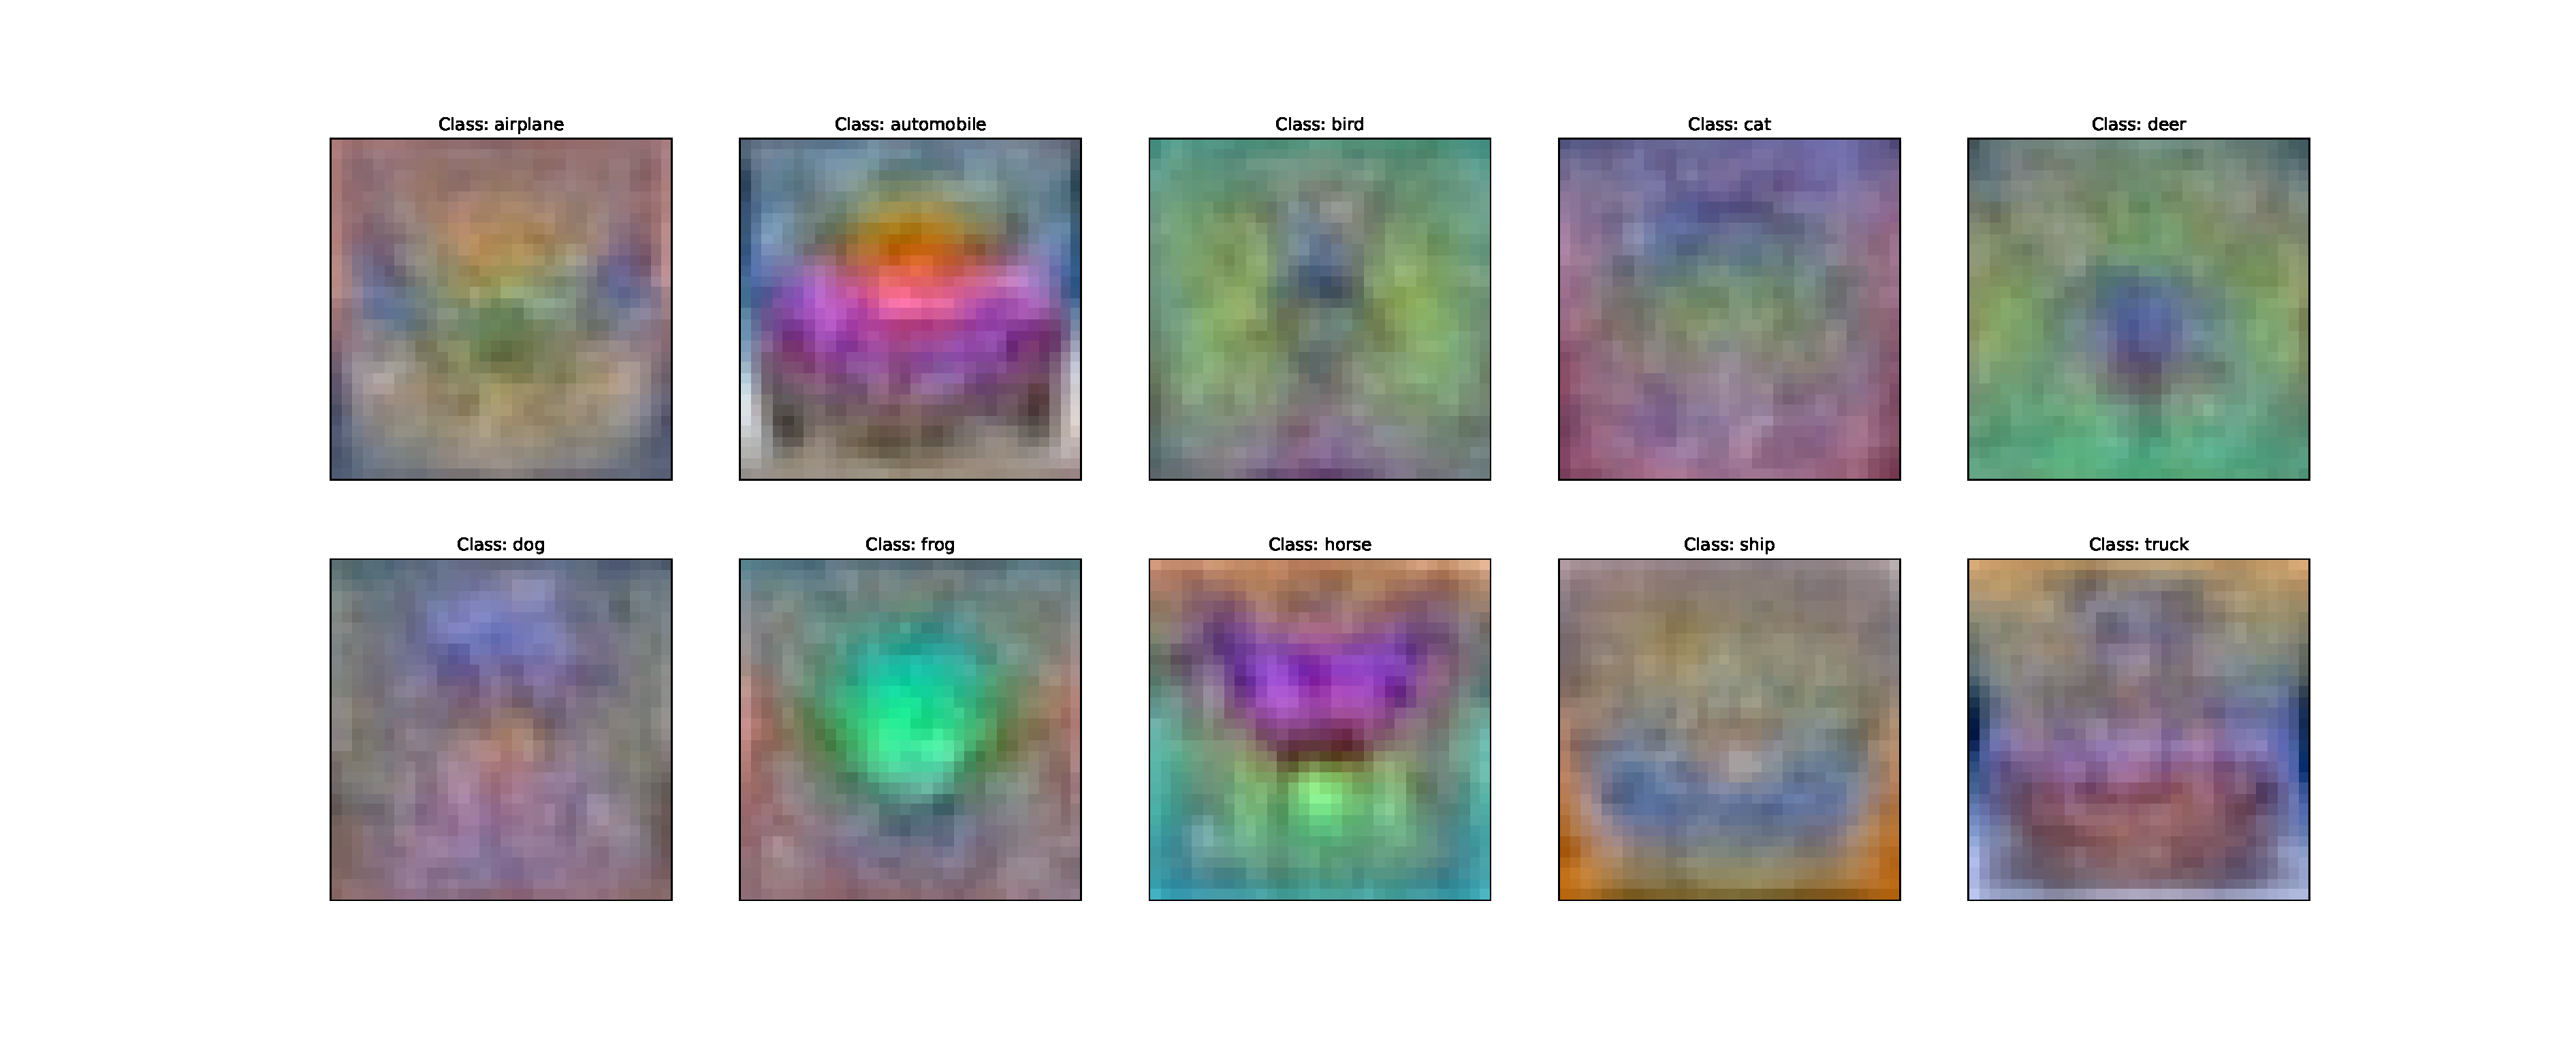
\includegraphics[scale=0.29]{figures/trainedWeightsp1}
	\caption{\footnotesize Weights matrix {\tt w1} as 10 images}
	\label{part1w}
\end{figure}

The learned weights at the end of learning for CIFAR-10 (after running the gradient descent 300 epochs), can be visualized as 10 figures in Fig. \ref{part1w}. Observe that, the weight matrix of the ``horse'' class slightly looks like a horse with two heads. This property is also visible in the ``automobile'' class too. Therefore theses templates will give maximum score for images of horses and automobiles respectively when the inner product is considered between the template and the image.\\

Hyperparameters of the  model, training and testing loss and accuracies corresponding to the first and last epochs are given below. Normalized losses and the accuracies are plot in the Fig. \ref{p1}.


\begin{verbatim}
	Initial Learning Rate = 1.4e-2, Learning Rate Decay = 0.999, Regularization Parameter = 5e-6
	Optimizer = Vanilla Gradient Descent(VGD), Epochs = 300
	
| Epoch 001 | Loss 0.5000 | accuracy: 0.0834 | val_loss: 0.4846 | val_accuracy: 0.2486 |
| Epoch 300 | Loss 0.3946 | accuracy: 0.4104 | val_loss: 0.3958 | val_accuracy: 0.3981 |
\end{verbatim}

\begin{figure}[!h]
	\centering
	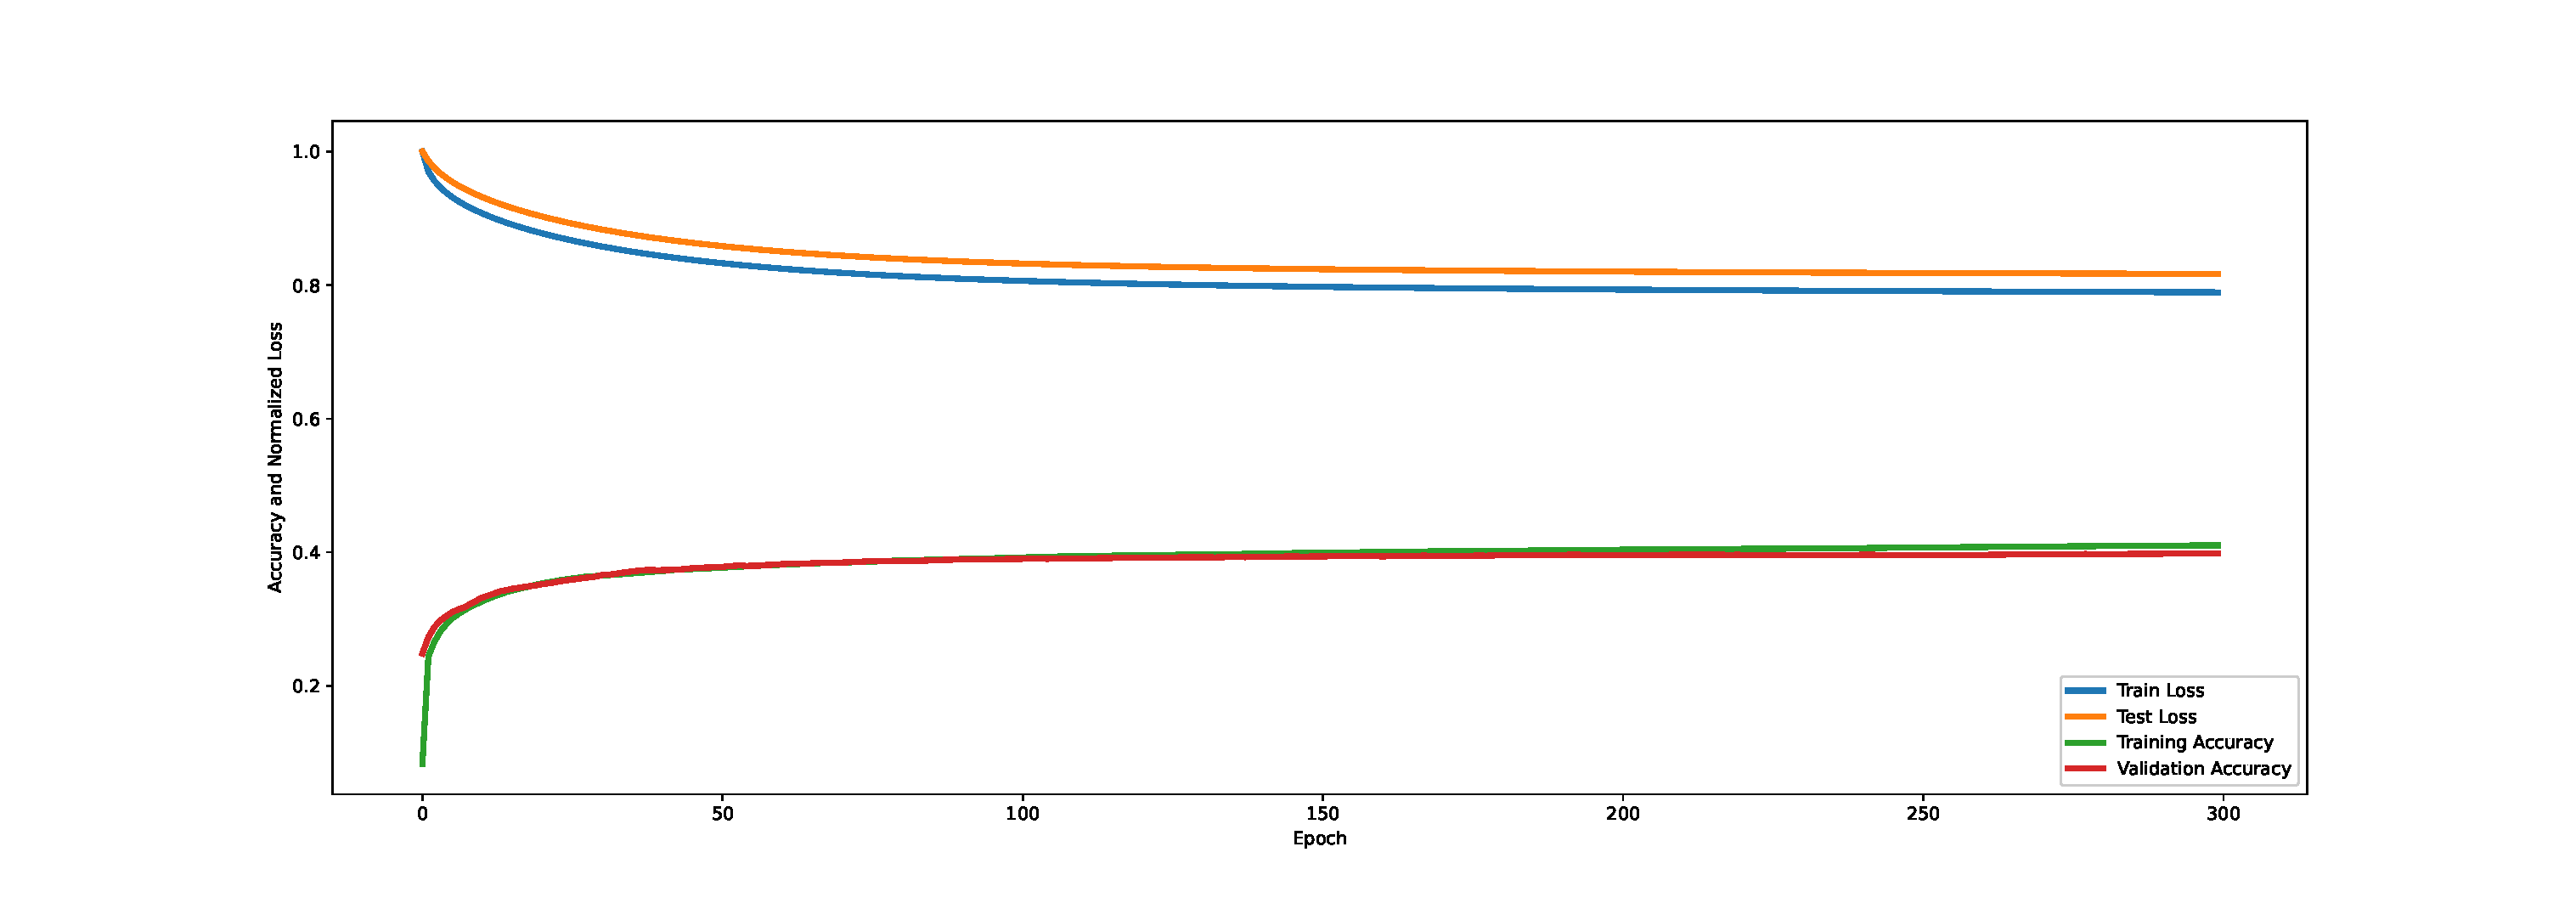
\includegraphics[scale=0.3]{figures/part1plots}
	\caption{\footnotesize Training Loss, Training Accuracy, Validation Loss and Validation Accuracy of the Linear Classifier with each iteration for 300 epochs}
	\label{p1}
\end{figure}

When observing the above figure following conclusions can be made. As the number of epochs increase, training and validation accuracies monotonically increase. But gap between the two curves also increases due to over-fitting of the model. Because parameters become more and more specific to the training set rather than become general to never seen images. The situation is the same for losses.\\

\hrule
\section*{Part 2}

As described in the part 1 weight matrices and bias vectors are concatenated into two matrices named {\tt w1} and {\tt w2}. The two layers are fully connected and  the {\tt sigmoid function} is used as the activation function for the hidden layer which consists of 200 hidden nodes. Layer 2, the output layer has no activation function.\\
\begin{tcolorbox}[breakable, size=fbox, boxrule=1pt, pad at break*=1mm,colback=cellbackground, colframe=cellborder]
\prompt{In}{incolor}{3}{\boxspacing}
\begin{Verbatim}[commandchars=\\\{\}]
\PY{n}{H} \PY{o}{=} \PY{l+m+mi}{200} \PY{c+c1}{\PYZsh{} No of hidden nodes}
\PY{n}{std}\PY{o}{=}\PY{l+m+mf}{1e\PYZhy{}5} 
\PY{c+c1}{\PYZsh{} Hidden Layer }
\PY{n}{w1} \PY{o}{=} \PY{n}{std}\PY{o}{*}\PY{n}{np}\PY{o}{.}\PY{n}{random}\PY{o}{.}\PY{n}{randn}\PY{p}{(}\PY{n}{Din}\PY{p}{,} \PY{n}{H}\PY{p}{)} \PY{c+c1}{\PYZsh{} Initializing the weight matrix with random weights}
\PY{n}{b1} \PY{o}{=} \PY{n}{np}\PY{o}{.}\PY{n}{zeros}\PY{p}{(}\PY{n}{H}\PY{p}{)} \PY{c+c1}{\PYZsh{} Initializing the bias vector}
\PY{c+c1}{\PYZsh{} Last Layer}
\PY{n}{w2} \PY{o}{=} \PY{n}{std}\PY{o}{*}\PY{n}{np}\PY{o}{.}\PY{n}{random}\PY{o}{.}\PY{n}{randn}\PY{p}{(}\PY{n}{H}\PY{p}{,} \PY{n}{K}\PY{p}{)} \PY{c+c1}{\PYZsh{} Initializing the weight matrix with random weights}
\PY{n}{b2} \PY{o}{=} \PY{n}{np}\PY{o}{.}\PY{n}{zeros}\PY{p}{(}\PY{n}{K}\PY{p}{)} \PY{c+c1}{\PYZsh{} Initializing the bias vector}
\PY{c+c1}{\PYZsh{} Rearranging train and test samples: (ra=rearranged)}
\PY{n}{x\PYZus{}train\PYZus{}ra} \PY{o}{=} \PY{n}{np}\PY{o}{.}\PY{n}{concatenate}\PY{p}{(}\PY{p}{(}\PY{n}{np}\PY{o}{.}\PY{n}{ones}\PY{p}{(}\PY{p}{(}\PY{n}{x\PYZus{}train}\PY{o}{.}\PY{n}{shape}\PY{p}{[}\PY{l+m+mi}{0}\PY{p}{]}\PY{p}{,}\PY{l+m+mi}{1}\PY{p}{)}\PY{p}{)}\PY{p}{,}\PY{n}{x\PYZus{}train}\PY{p}{)}\PY{p}{,} \PY{n}{axis}\PY{o}{=}\PY{l+m+mi}{1}\PY{p}{)}
\PY{n}{x\PYZus{}test\PYZus{}ra}  \PY{o}{=} \PY{n}{np}\PY{o}{.}\PY{n}{concatenate}\PY{p}{(}\PY{p}{(}\PY{n}{np}\PY{o}{.}\PY{n}{ones}\PY{p}{(}\PY{p}{(}\PY{n}{x\PYZus{}test}\PY{o}{.}\PY{n}{shape}\PY{p}{[}\PY{l+m+mi}{0}\PY{p}{]}\PY{p}{,}\PY{l+m+mi}{1}\PY{p}{)}\PY{p}{)}\PY{p}{,}\PY{n}{x\PYZus{}test}\PY{p}{)}\PY{p}{,} \PY{n}{axis}\PY{o}{=}\PY{l+m+mi}{1}\PY{p}{)}
\PY{c+c1}{\PYZsh{} Rearranging weight matrices and bias vectors into single matrices}
\PY{n}{w1} \PY{o}{=} \PY{n}{np}\PY{o}{.}\PY{n}{concatenate}\PY{p}{(}\PY{p}{(}\PY{n}{b1}\PY{o}{.}\PY{n}{reshape}\PY{p}{(}\PY{l+m+mi}{1}\PY{p}{,}\PY{n}{H}\PY{p}{)}\PY{p}{,} \PY{n}{w1}\PY{p}{)}\PY{p}{,} \PY{n}{axis}\PY{o}{=}\PY{l+m+mi}{0}\PY{p}{)}
\PY{n}{w2} \PY{o}{=} \PY{n}{np}\PY{o}{.}\PY{n}{concatenate}\PY{p}{(}\PY{p}{(}\PY{n}{b2}\PY{o}{.}\PY{n}{reshape}\PY{p}{(}\PY{l+m+mi}{1}\PY{p}{,}\PY{n}{K}\PY{p}{)}\PY{p}{,} \PY{n}{w2}\PY{p}{)}\PY{p}{,} \PY{n}{axis}\PY{o}{=}\PY{l+m+mi}{0}\PY{p}{)}
\end{Verbatim}
\end{tcolorbox}

\textbf{\textit{Normalization of image pixel values was removed from the data pre-processing stage}} as it was observed that model stops learning after few iterations. Because extremely small weights in the matrices, keeps the weight matrices almost the same and the change in loss function becomes negligible.

The loss function used in the part 1 is used here as well, with the additional term related to the {\tt w2} matrix.
{ \scriptsize\[
	\therefore ~ Loss~ Function = \frac{1}{2m}.\sum\left[ \left( hypothesis - y_{train}\right)^2 + \lambda W_1^2 + \lambda W_2^2 \right]~ where~\lambda = regularization~parameter
	\]}


    \begin{tcolorbox}[breakable, size=fbox, boxrule=1pt, pad at break*=1mm,colback=cellbackground, colframe=cellborder]
\prompt{In}{incolor}{4}{\boxspacing}
\begin{Verbatim}[commandchars=\\\{\}]
\PY{k}{for} \PY{n}{t} \PY{o+ow}{in} \PY{n+nb}{range}\PY{p}{(}\PY{l+m+mi}{1}\PY{p}{,}\PY{n}{iterations}\PY{o}{+}\PY{l+m+mi}{1}\PY{p}{)}\PY{p}{:}
    \PY{c+c1}{\PYZsh{} Forward Propagation}
    \PY{n}{hypo} \PY{o}{=} \PY{n}{sigmoid}\PY{p}{(}\PY{n}{x\PYZus{}train\PYZus{}ra}\PY{o}{.}\PY{n}{dot}\PY{p}{(}\PY{n}{w1}\PY{p}{)}\PY{p}{)} \PY{c+c1}{\PYZsh{} Layer 1 with sigmoid activation}
    \PY{n}{hypothesis} \PY{o}{=} \PY{n}{np}\PY{o}{.}\PY{n}{concatenate}\PY{p}{(}\PY{p}{(}\PY{n}{np}\PY{o}{.}\PY{n}{ones}\PY{p}{(}\PY{p}{(}\PY{n}{hypo}\PY{o}{.}\PY{n}{shape}\PY{p}{[}\PY{l+m+mi}{0}\PY{p}{]}\PY{p}{,}\PY{l+m+mi}{1}\PY{p}{)}\PY{p}{)}\PY{p}{,}\PY{n}{hypo}\PY{p}{)}\PY{p}{,} \PY{n}{axis}\PY{o}{=}\PY{l+m+mi}{1}\PY{p}{)} \PY{c+c1}{\PYZsh{} Rearranging for layer 2}
    \PY{n}{predict} \PY{o}{=} \PY{n}{hypothesis}\PY{o}{.}\PY{n}{dot}\PY{p}{(}\PY{n}{w2}\PY{p}{)} \PY{c+c1}{\PYZsh{} Layer 2     }
    \PY{n}{loss} \PY{o}{=} \PY{p}{(}\PY{l+m+mi}{1}\PY{o}{/}\PY{p}{(}\PY{l+m+mi}{2}\PY{o}{*}\PY{n}{m}\PY{p}{)}\PY{p}{)}\PY{o}{*}\PY{n}{np}\PY{o}{.}\PY{n}{sum}\PY{p}{(}\PY{p}{(} \PY{n}{predict} \PY{o}{\PYZhy{}} \PY{n}{y\PYZus{}train}\PY{p}{)}\PY{o}{*}\PY{o}{*}\PY{l+m+mi}{2}\PY{p}{)}\PYZbs{}
         \PY{o}{+} \PY{p}{(}\PY{l+m+mi}{1}\PY{o}{/}\PY{p}{(}\PY{l+m+mi}{2}\PY{o}{*}\PY{n}{m}\PY{p}{)}\PY{p}{)}\PY{o}{*}\PY{n}{reg}\PY{o}{*}\PY{n}{np}\PY{o}{.}\PY{n}{sum}\PY{p}{(}\PY{n}{w1}\PY{o}{*}\PY{o}{*}\PY{l+m+mi}{2}\PY{p}{)} \PY{o}{+} \PY{p}{(}\PY{l+m+mi}{1}\PY{o}{/}\PY{p}{(}\PY{l+m+mi}{2}\PY{o}{*}\PY{n}{m}\PY{p}{)}\PY{p}{)}\PY{o}{*}\PY{n}{reg}\PY{o}{*}\PY{n}{np}\PY{o}{.}\PY{n}{sum}\PY{p}{(}\PY{n}{w2}\PY{o}{*}\PY{o}{*}\PY{l+m+mi}{2}\PY{p}{)}
    \PY{c+c1}{\PYZsh{} Back Propagation: partial dertivatives of Loss function}
    \PY{n}{dpredict} \PY{o}{=}  \PY{p}{(}\PY{l+m+mi}{1}\PY{o}{/}\PY{n}{m}\PY{p}{)}\PY{o}{*}\PY{p}{(}\PY{n}{predict} \PY{o}{\PYZhy{}} \PY{n}{y\PYZus{}train}\PY{p}{)}
    \PY{n}{dw2} \PY{o}{=} \PY{n}{hypothesis}\PY{o}{.}\PY{n}{T}\PY{o}{.}\PY{n}{dot}\PY{p}{(}\PY{n}{dpredict}\PY{p}{)} \PY{o}{+} \PY{p}{(}\PY{l+m+mi}{1}\PY{o}{/}\PY{n}{m}\PY{p}{)}\PY{o}{*}\PY{n}{reg}\PY{o}{*}\PY{n}{w2}
    \PY{n}{dh} \PY{o}{=} \PY{n}{dpredict}\PY{o}{.}\PY{n}{dot}\PY{p}{(}\PY{n}{w2}\PY{p}{[}\PY{l+m+mi}{1}\PY{p}{:}\PY{p}{,}\PY{p}{]}\PY{o}{.}\PY{n}{T}\PY{p}{)} \PY{c+c1}{\PYZsh{} Removing bias vector w2(201 X 10)\PYZhy{}\PYZhy{}\PYZgt{} 200 X 10}
    \PY{n}{dhdxw1} \PY{o}{=} \PY{n}{hypo}\PY{o}{*}\PY{p}{(}\PY{l+m+mi}{1} \PY{o}{\PYZhy{}} \PY{n}{hypo}\PY{p}{)} \PY{c+c1}{\PYZsh{}using the hypothesis(50000X200), the one before rearranging.}
    \PY{n}{dw1} \PY{o}{=} \PY{n}{x\PYZus{}train\PYZus{}ra}\PY{o}{.}\PY{n}{T}\PY{o}{.}\PY{n}{dot}\PY{p}{(}\PY{n}{dh}\PY{o}{*}\PY{n}{dhdxw1}\PY{p}{)} \PY{o}{+} \PY{p}{(}\PY{l+m+mi}{1}\PY{o}{/}\PY{n}{m}\PY{p}{)}\PY{o}{*}\PY{n}{reg}\PY{o}{*}\PY{n}{w1}    
    \PY{c+c1}{\PYZsh{} Gradient Descent}
    \PY{n}{w1} \PY{o}{=} \PY{n}{w1} \PY{o}{\PYZhy{}} \PY{n}{lr}\PY{o}{*}\PY{n}{dw1}
    \PY{n}{w2} \PY{o}{=} \PY{n}{w2} \PY{o}{\PYZhy{}} \PY{n}{lr}\PY{o}{*}\PY{n}{dw2}
     \PY{c+c1}{\PYZsh{} Decaying learning rate}
    \PY{n}{lr} \PY{o}{=} \PY{n}{lr}\PY{o}{*}\PY{n}{lr\PYZus{}decay}
\end{Verbatim}
\end{tcolorbox}

\begin{verbatim}
	Initial Learning Rate = 1.4e-2, Learning Rate Decay = 0.999, Regularization Parameter = 5e-6 
	Optimizer = Vanilla Gradient Descent(VGD), Epochs = 300
	
	| Epoch 001 | Loss 0.5000 | accuracy: 0.1000 | val_loss: 0.4541 | val_accuracy: 0.1339 |
	| Epoch 300 | Loss 0.3765 | accuracy: 0.4436 | val_loss: 0.3813 | val_accuracy: 0.4275 |
\end{verbatim}


\begin{figure}[!h]
	\centering
	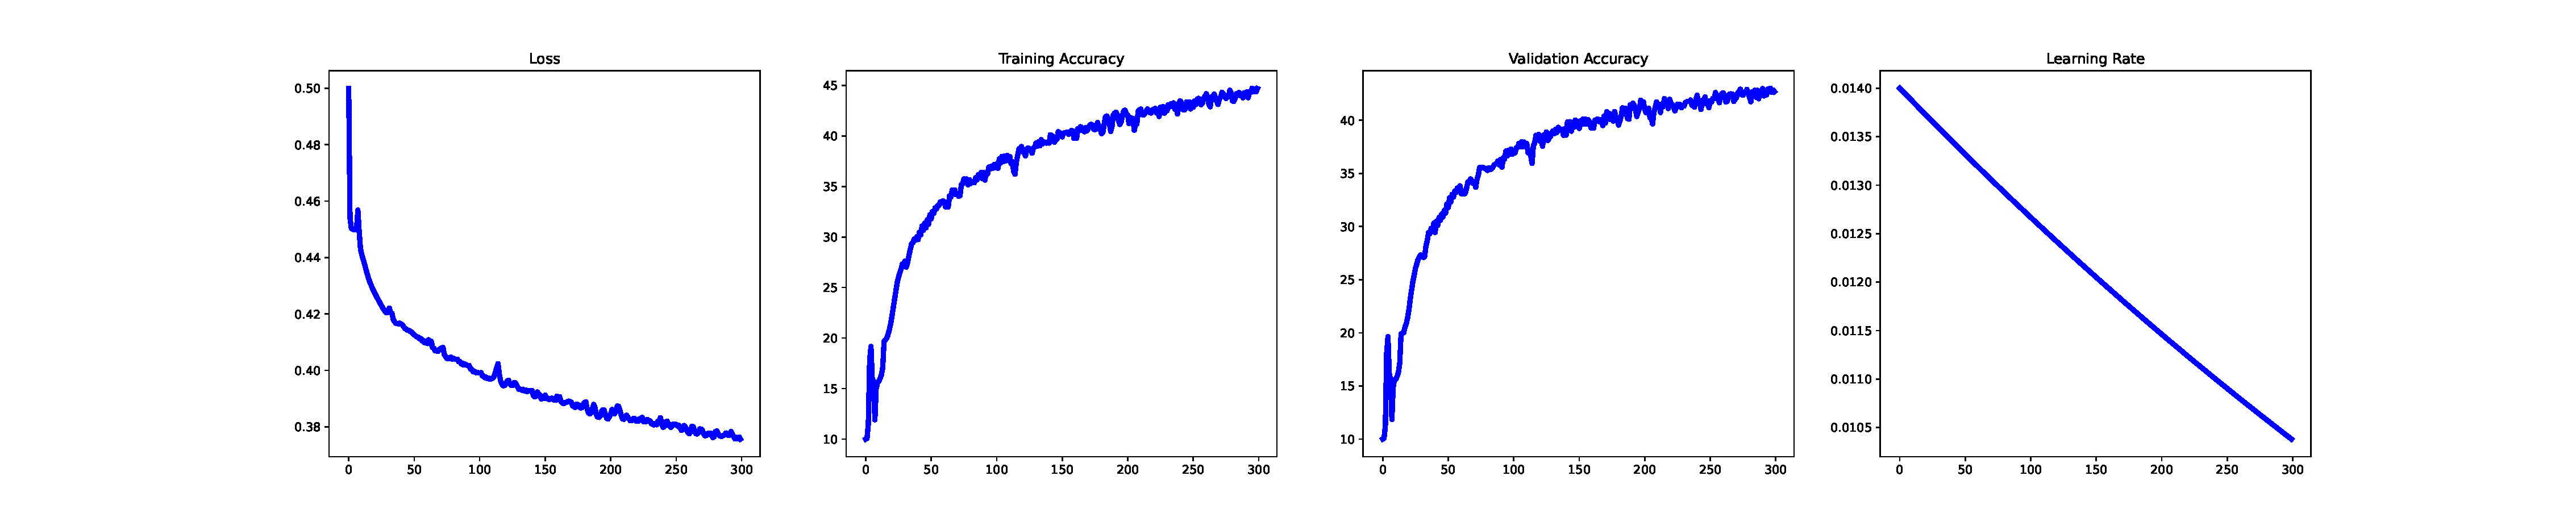
\includegraphics[scale=0.3]{figures/part2plots}
	\caption{\footnotesize Training Loss, Training Accuracy, Validation Loss and Validation Accuracy of the 2 Layer Classifier with each iteration:  for 300 epochs}
\end{figure}

As described in the part 1 the same reason applies for the behavior of the gaps between normalized losses and accuracies curves. In addition to that due to the non linearity introduced by the {\tt sigmoid function} at the hidden nodes, curves are not smooth as they were in the part 1 linear classifier.\\

\hrule
\section*{Part 3}

For the purpose of comparison hyperparameters were kept the same as in part 2. But the optimizer changes form Vanilla Gradient Descent to Mini-batch Gradient Descent(mentioned as stochastic GD-SGD).

\begin{verbatim}
	Initial Learning Rate = 1.4e-2, Learning Rate Decay = 0.999, Regularization Parameter = 5e-6
	Optimizer = Mini Batch Gradient Descent, Batch Size = 500, Epochs = 300
	
| Epoch 001 | Loss 0.4768 | accuracy: 0.1249 | val_loss: 0.4619 | val_accuracy: 0.1252 |
| Epoch 300 | Loss 0.3686 | accuracy: 0.4674 | val_loss: 0.3768 | val_accuracy: 0.4432 |
\end{verbatim}


\begin{figure}[!h]
	\centering
	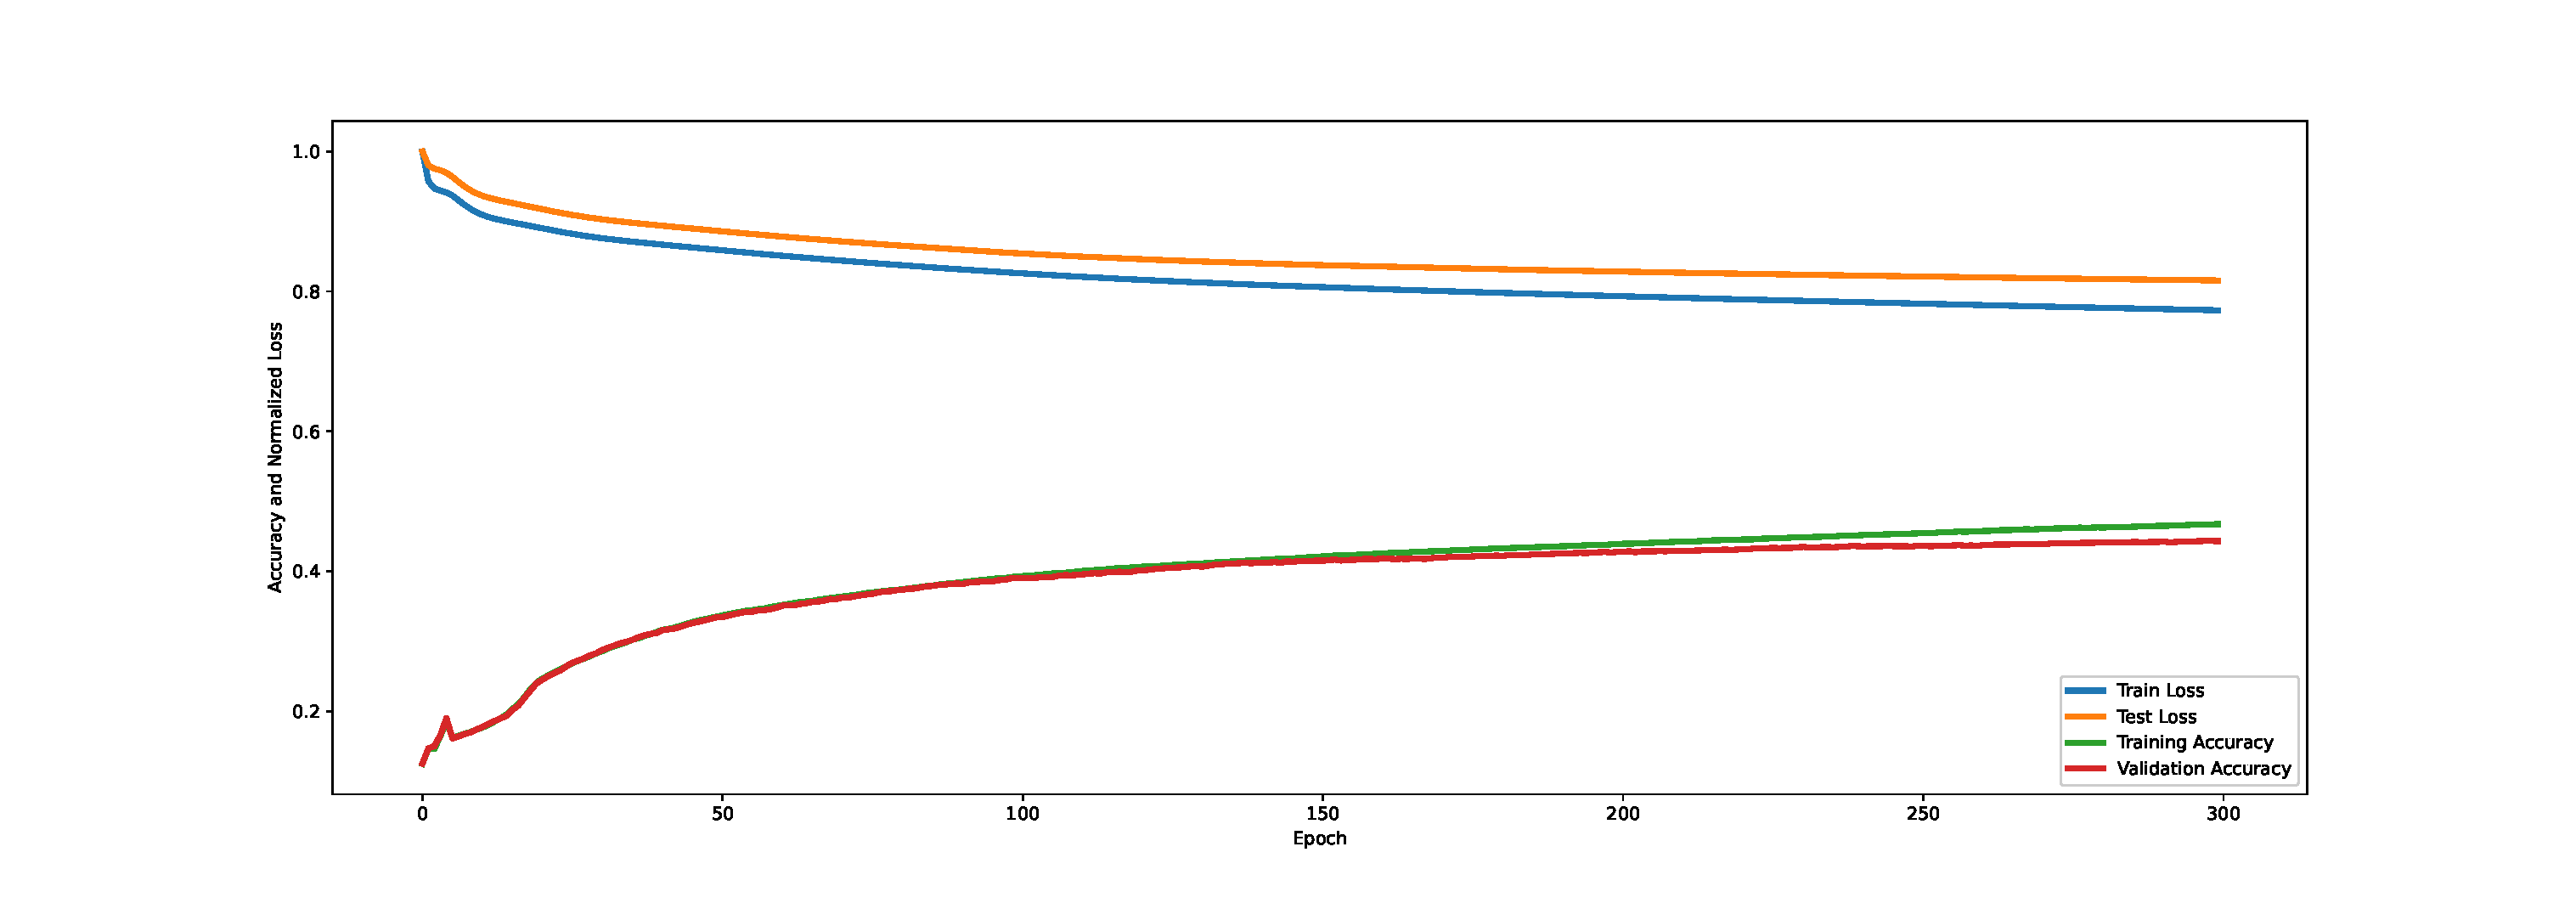
\includegraphics[scale=0.3]{figures/part3plots}
	\caption{\footnotesize Training Loss, Training Accuracy, Validation Loss and Validation Accuracy of the 2 Layer Classifier with each iteration for 300 epochs: Using Mini Batch Gradient Descent as the optimizer}
\end{figure}

consider the accuracies and losses related to the last epochs of the Part 2 and Part 3. 
\begin{verbatim}
	| VGD | Epoch 300 | Loss 0.3765 | accuracy: 0.4436 | val_loss: 0.3813 | val_accuracy: 0.4275 |
	| SGD | Epoch 300 | Loss 0.3686 | accuracy: 0.4674 | val_loss: 0.3768 | val_accuracy: 0.4432 |	
\end{verbatim}
In Part 2  \textbf{the same batch}(50,000) training samples were used \textbf{\textit{for every step of Gradient Descent}} and therefore the parameters become more specific to the training set as there is no any randomness in the data processed in each iteration. But with the Mini batch GD optimizer it is not the case. At each epoch the training set(50,000) is \textbf{\textit{shuffled}} and  \textbf{\textit{divided into}} number($n = \frac{Number~ of~ Training~ samples}{Batch~size}$) of \textit{\textbf{mini batches}}. After that gradient descent is carried out on each such mini batch and weights are updated accordingly. The advantage of this process is, since the batch is shuffled and only a small set of the batch is seen by the model at one gradient descent step, it performs well on the never seen test samples better than the algorithm in part 2. 

    \begin{tcolorbox}[breakable, size=fbox, boxrule=1pt, pad at break*=1mm,colback=cellbackground, colframe=cellborder]
\prompt{In}{incolor}{5}{\boxspacing}
\begin{Verbatim}[commandchars=\\\{\}]
\PY{n}{batch\PYZus{}size} \PY{o}{=} \PY{l+m+mi}{500} \PY{c+c1}{\PYZsh{} define the batch size}
\PY{n}{seed} \PY{o}{=} \PY{l+m+mi}{0}\PY{p}{;} \PY{n}{rng} \PY{o}{=} \PY{n}{np}\PY{o}{.}\PY{n}{random}\PY{o}{.}\PY{n}{default\PYZus{}rng}\PY{p}{(}\PY{n}{seed}\PY{o}{=}\PY{n}{seed}\PY{p}{)}
\PY{k}{for} \PY{n}{t} \PY{o+ow}{in} \PY{n+nb}{range}\PY{p}{(}\PY{l+m+mi}{1}\PY{p}{,}\PY{n}{iterations}\PY{o}{+}\PY{l+m+mi}{1}\PY{p}{)}\PY{p}{:}
    \PY{n}{indices} \PY{o}{=} \PY{n}{np}\PY{o}{.}\PY{n}{arange}\PY{p}{(}\PY{n}{Ntr}\PY{p}{)} \PY{c+c1}{\PYZsh{}Number of training samples}
    \PY{n}{rng}\PY{o}{.}\PY{n}{shuffle}\PY{p}{(}\PY{n}{indices}\PY{p}{)}
    \PY{n}{x\PYZus{}train\PYZus{}3} \PY{o}{=} \PY{n}{x\PYZus{}train\PYZus{}ra}\PY{p}{[}\PY{n}{indices}\PY{p}{]}
    \PY{n}{y\PYZus{}train\PYZus{}3} \PY{o}{=} \PY{n}{y\PYZus{}train}\PY{p}{[}\PY{n}{indices}\PY{p}{]}
    \PY{n}{batch\PYZus{}loss} \PY{o}{=} \PY{l+m+mi}{0} \PY{c+c1}{\PYZsh{} Loss for each batch}
    \PY{k}{for} \PY{n}{start} \PY{o+ow}{in} \PY{n+nb}{range}\PY{p}{(}\PY{l+m+mi}{0}\PY{p}{,}\PY{n}{Ntr}\PY{p}{,}\PY{n}{batch\PYZus{}size}\PY{p}{)}\PY{p}{:}
        \PY{n}{stop} \PY{o}{=} \PY{n}{start} \PY{o}{+} \PY{n}{batch\PYZus{}size}
        \PY{c+c1}{\PYZsh{} Forward Propagation}
        \PY{n}{hypo} \PY{o}{=} \PY{n}{sigmoid}\PY{p}{(}\PY{n}{x\PYZus{}train\PYZus{}3}\PY{p}{[}\PY{n}{start}\PY{p}{:}\PY{n}{stop}\PY{p}{]}\PY{o}{.}\PY{n}{dot}\PY{p}{(}\PY{n}{w1}\PY{p}{)}\PY{p}{)} \PY{c+c1}{\PYZsh{} Layer 1 with sigmoid activation}
        \PY{n}{hypothesis} \PY{o}{=} \PY{n}{np}\PY{o}{.}\PY{n}{concatenate}\PY{p}{(}\PY{p}{(}\PY{n}{np}\PY{o}{.}\PY{n}{ones}\PY{p}{(}\PY{p}{(}\PY{n}{hypo}\PY{o}{.}\PY{n}{shape}\PY{p}{[}\PY{l+m+mi}{0}\PY{p}{]}\PY{p}{,}\PY{l+m+mi}{1}\PY{p}{)}\PY{p}{)}\PY{p}{,}\PY{n}{hypo}\PY{p}{)}\PY{p}{,} \PY{n}{axis}\PY{o}{=}\PY{l+m+mi}{1}\PY{p}{)}
        \PY{n}{predict} \PY{o}{=} \PY{n}{hypothesis}\PY{o}{.}\PY{n}{dot}\PY{p}{(}\PY{n}{w2}\PY{p}{)} \PY{c+c1}{\PYZsh{} Layer 2 }
        \PY{n}{minibatch\PYZus{}loss} \PY{o}{=} \PY{p}{(}\PY{l+m+mi}{1}\PY{o}{/}\PY{p}{(}\PY{l+m+mi}{2}\PY{o}{*}\PY{n}{m}\PY{p}{)}\PY{p}{)}\PY{o}{*}\PY{n}{np}\PY{o}{.}\PY{n}{sum}\PY{p}{(}\PY{p}{(} \PY{n}{predict} \PY{o}{\PYZhy{}} \PY{n}{y\PYZus{}train\PYZus{}3}\PY{p}{[}\PY{n}{start}\PY{p}{:}\PY{n}{stop}\PY{p}{]}\PY{p}{)}\PY{o}{*}\PY{o}{*}\PY{l+m+mi}{2}\PY{p}{)}\PYZbs{}
             \PY{o}{+} \PY{p}{(}\PY{l+m+mi}{1}\PY{o}{/}\PY{p}{(}\PY{l+m+mi}{2}\PY{o}{*}\PY{n}{m}\PY{p}{)}\PY{p}{)}\PY{o}{*}\PY{n}{reg}\PY{o}{*}\PY{n}{np}\PY{o}{.}\PY{n}{sum}\PY{p}{(}\PY{n}{w1}\PY{o}{*}\PY{o}{*}\PY{l+m+mi}{2}\PY{p}{)} \PY{o}{+} \PY{p}{(}\PY{l+m+mi}{1}\PY{o}{/}\PY{p}{(}\PY{l+m+mi}{2}\PY{o}{*}\PY{n}{m}\PY{p}{)}\PY{p}{)}\PY{o}{*}\PY{n}{reg}\PY{o}{*}\PY{n}{np}\PY{o}{.}\PY{n}{sum}\PY{p}{(}\PY{n}{w2}\PY{o}{*}\PY{o}{*}\PY{l+m+mi}{2}\PY{p}{)}
        \PY{n}{batch\PYZus{}loss}\PY{o}{+}\PY{o}{=} \PY{n}{minibatch\PYZus{}loss}
        \PY{c+c1}{\PYZsh{} Back Propagation partial dertivatives of Loss function}
        \PY{n}{dpredict} \PY{o}{=}  \PY{p}{(}\PY{l+m+mi}{1}\PY{o}{/}\PY{n}{m}\PY{p}{)}\PY{o}{*}\PY{p}{(}\PY{n}{predict} \PY{o}{\PYZhy{}} \PY{n}{y\PYZus{}train\PYZus{}3}\PY{p}{[}\PY{n}{start}\PY{p}{:}\PY{n}{stop}\PY{p}{]}\PY{p}{)}
        \PY{n}{dw2} \PY{o}{=} \PY{n}{hypothesis}\PY{o}{.}\PY{n}{T}\PY{o}{.}\PY{n}{dot}\PY{p}{(}\PY{n}{dpredict}\PY{p}{)} \PY{o}{+} \PY{p}{(}\PY{l+m+mi}{1}\PY{o}{/}\PY{n}{m}\PY{p}{)}\PY{o}{*}\PY{n}{reg}\PY{o}{*}\PY{n}{w2}
        \PY{n}{dh} \PY{o}{=} \PY{n}{dpredict}\PY{o}{.}\PY{n}{dot}\PY{p}{(}\PY{n}{w2}\PY{p}{[}\PY{l+m+mi}{1}\PY{p}{:}\PY{p}{,}\PY{p}{]}\PY{o}{.}\PY{n}{T}\PY{p}{)} \PY{c+c1}{\PYZsh{} Removing bias vector w2(201x10)\PYZhy{}\PYZhy{}\PYZgt{} 200x10}
        \PY{n}{dhdxw1} \PY{o}{=} \PY{n}{hypo}\PY{o}{*}\PY{p}{(}\PY{l+m+mi}{1} \PY{o}{\PYZhy{}} \PY{n}{hypo}\PY{p}{)} \PY{c+c1}{\PYZsh{}using hypothesis 50000*200, the one before rearranging.}
        \PY{n}{dw1} \PY{o}{=} \PY{n}{x\PYZus{}train\PYZus{}3}\PY{p}{[}\PY{n}{start}\PY{p}{:}\PY{n}{stop}\PY{p}{]}\PY{o}{.}\PY{n}{T}\PY{o}{.}\PY{n}{dot}\PY{p}{(}\PY{n}{dh}\PY{o}{*}\PY{n}{dhdxw1}\PY{p}{)} \PY{o}{+} \PY{p}{(}\PY{l+m+mi}{1}\PY{o}{/}\PY{n}{m}\PY{p}{)}\PY{o}{*}\PY{n}{reg}\PY{o}{*}\PY{n}{w1}
        \PY{n}{w1} \PY{o}{=} \PY{n}{w1} \PY{o}{\PYZhy{}} \PY{n}{lr}\PY{o}{*}\PY{n}{dw1}  \PY{c+c1}{\PYZsh{} Gradient Descent}
        \PY{n}{w2} \PY{o}{=} \PY{n}{w2} \PY{o}{\PYZhy{}} \PY{n}{lr}\PY{o}{*}\PY{n}{dw2}  \PY{c+c1}{\PYZsh{} Gradient Descent}
    \PY{n}{lr} \PY{o}{=} \PY{n}{lr}\PY{o}{*}\PY{n}{lr\PYZus{}decay}      \PY{c+c1}{\PYZsh{} Decaying the learning rate}
\end{Verbatim}
\end{tcolorbox}


\section*{Part 4}

The CNN model declared below starts over-fitting around the $8^{th}$ epoch. Therefore the number of epochs was limited to 10. This fact is clearly visible, because at the $10^{th}$ epoch even though the training loss and accuracy are better than that of the $8^{th}$ epoch, validation loss and validation accuracy are worse. However, the model has performed absolutely better than any of the previous models in 8 epochs with a validation accuracy of $69.79\%$. Previously we were only able to reach up to $44.32\%$ of validation accuracy with the defined hyperparameters.


\begin{verbatim}
	Initial Learning Rate = 1.4e-2,  Learnable Parameters: 73,418
	Optimizer = SGD with Momentum = 0.9, Batch Size = 50, Epochs = 10
	
	| Epoch 001 | Loss: 1.8674 | accuracy: 0.3070 | val_loss: 1.2984 | val_accuracy: 0.5298 |
	| Epoch 008 | Loss: 0.6375 | accuracy: 0.7746 | val_loss: 0.8601 | val_accuracy: 0.7088 |
	| Epoch 010 | Loss: 0.5651 | accuracy: 0.8021 | val_loss: 0.9394 | val_accuracy: 0.6979 |
\end{verbatim}


\begin{figure}[!h]
	\centering
	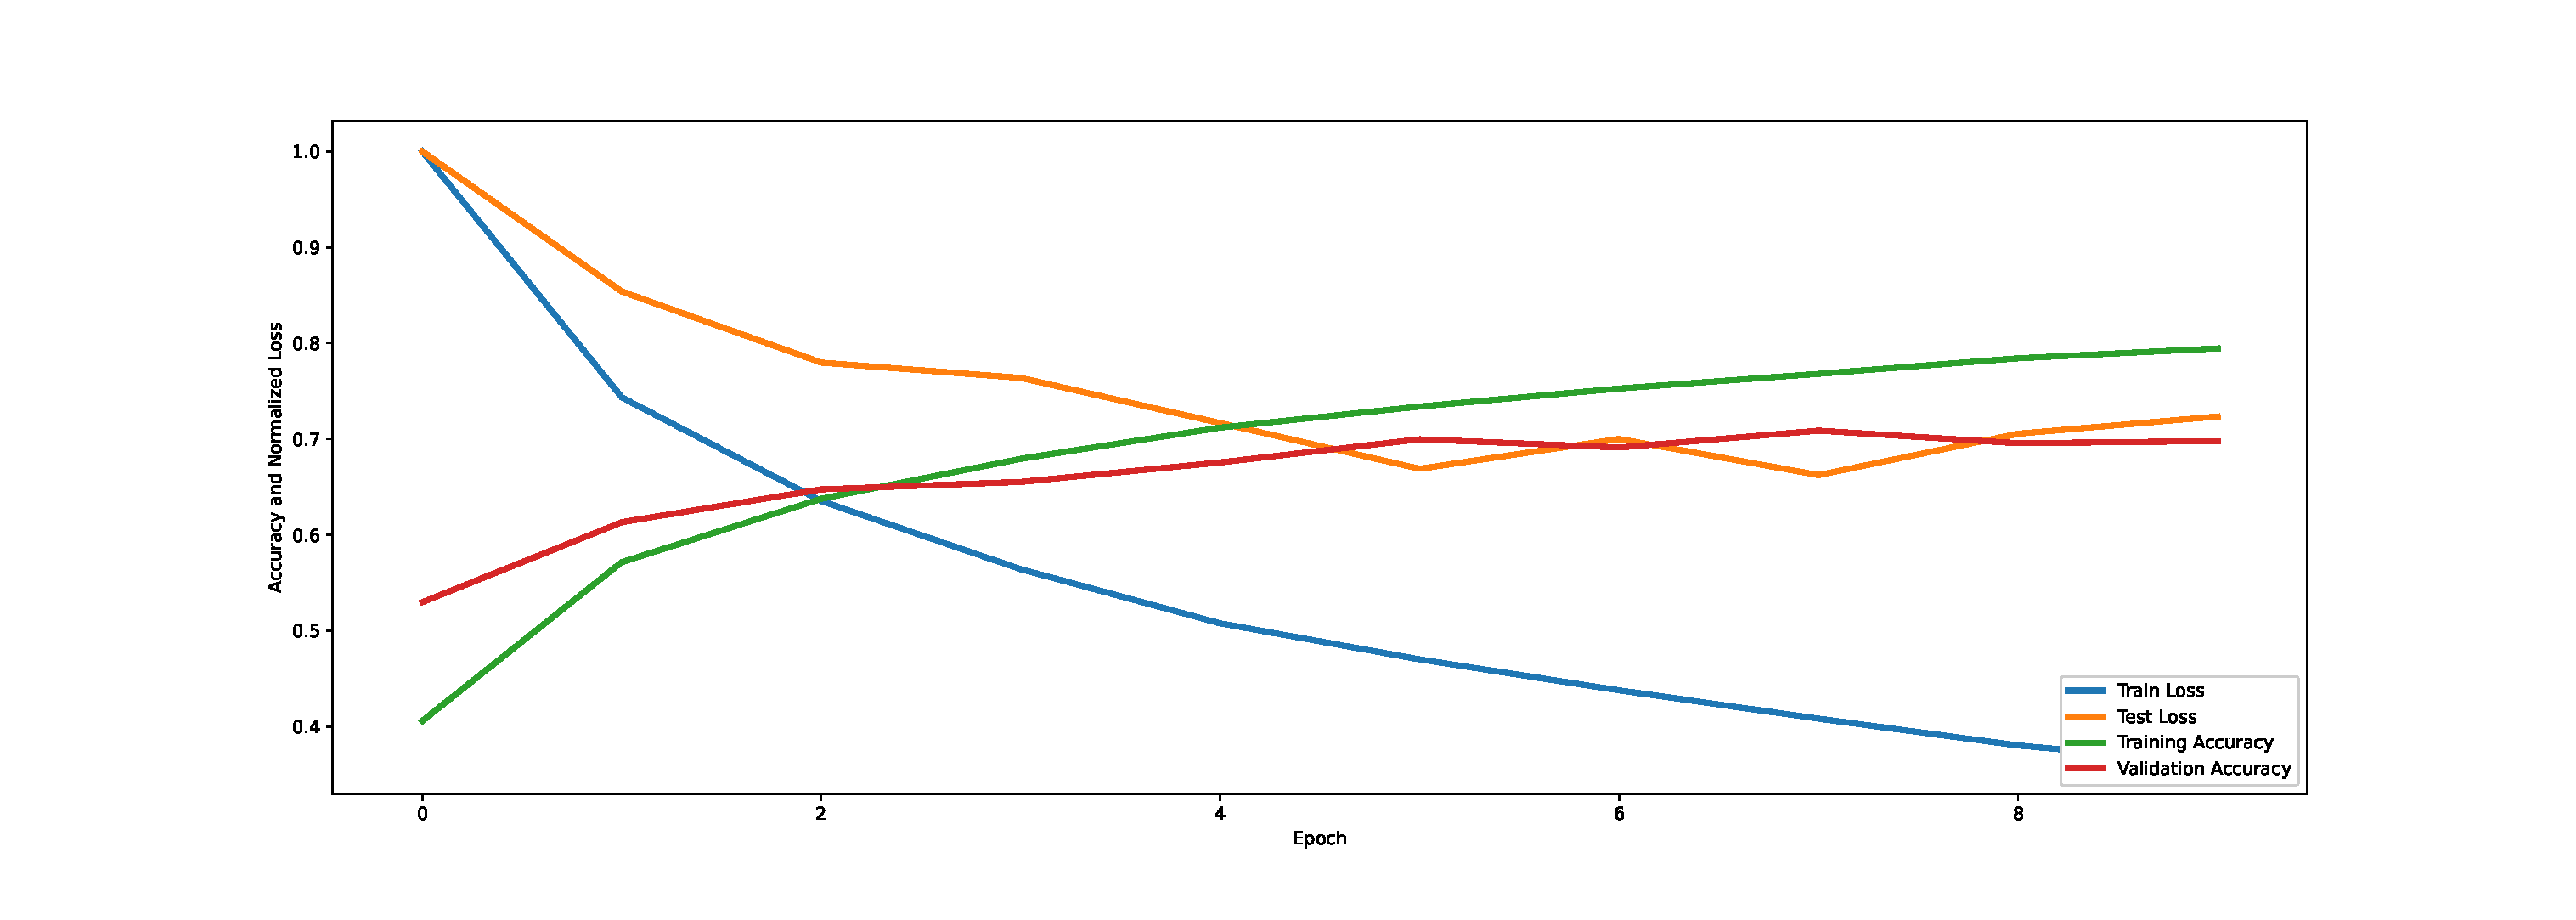
\includegraphics[scale=0.3]{figures/part4plots}
	\caption{\footnotesize Training Loss, Training Accuracy, Validation Loss and Validation Accuracy of the CNN model}
\end{figure}

    \begin{tcolorbox}[breakable, size=fbox, boxrule=1pt, pad at break*=1mm,colback=cellbackground, colframe=cellborder]
\prompt{In}{incolor}{6}{\boxspacing}
\begin{Verbatim}[commandchars=\\\{\}]
\PY{p}{(}\PY{n}{x\PYZus{}train}\PY{p}{,} \PY{n}{y\PYZus{}train}\PY{p}{)}\PY{p}{,} \PY{p}{(}\PY{n}{x\PYZus{}test}\PY{p}{,} \PY{n}{y\PYZus{}test}\PY{p}{)} \PY{o}{=} \PY{n}{datasets}\PY{o}{.}\PY{n}{cifar10}\PY{o}{.}\PY{n}{load\PYZus{}data}\PY{p}{(}\PY{p}{)}
\PY{n}{K} \PY{o}{=} \PY{n+nb}{len}\PY{p}{(}\PY{n}{np}\PY{o}{.}\PY{n}{unique}\PY{p}{(}\PY{n}{y\PYZus{}train}\PY{p}{)}\PY{p}{)} \PY{c+c1}{\PYZsh{} Number of Classes}
\PY{c+c1}{\PYZsh{} Normalize pixel values: Image data preprocessing}
\PY{n}{x\PYZus{}train}\PY{p}{,} \PY{n}{x\PYZus{}test} \PY{o}{=} \PY{n}{x\PYZus{}train} \PY{o}{/} \PY{l+m+mf}{255.0}\PY{p}{,} \PY{n}{x\PYZus{}test} \PY{o}{/} \PY{l+m+mf}{255.0}
\PY{n}{mean\PYZus{}image} \PY{o}{=} \PY{n}{np}\PY{o}{.}\PY{n}{mean}\PY{p}{(}\PY{n}{x\PYZus{}train}\PY{p}{,} \PY{n}{axis}\PY{o}{=}\PY{l+m+mi}{0}\PY{p}{)} \PY{c+c1}{\PYZsh{} axis=0: mean of a column; Mean of each pixel}
\PY{n}{x\PYZus{}train} \PY{o}{=} \PY{n}{x\PYZus{}train} \PY{o}{\PYZhy{}} \PY{n}{mean\PYZus{}image}
\PY{n}{x\PYZus{}test} \PY{o}{=} \PY{n}{x\PYZus{}test} \PY{o}{\PYZhy{}} \PY{n}{mean\PYZus{}image}
\PY{c+c1}{\PYZsh{} Convert class vectors to binary class matrices.}
\PY{n}{y\PYZus{}train} \PY{o}{=} \PY{n}{tf}\PY{o}{.}\PY{n}{keras}\PY{o}{.}\PY{n}{utils}\PY{o}{.}\PY{n}{to\PYZus{}categorical}\PY{p}{(}\PY{n}{y\PYZus{}train}\PY{p}{,} \PY{n}{num\PYZus{}classes}\PY{o}{=}\PY{n}{K}\PY{p}{)}
\PY{n}{y\PYZus{}test} \PY{o}{=} \PY{n}{tf}\PY{o}{.}\PY{n}{keras}\PY{o}{.}\PY{n}{utils}\PY{o}{.}\PY{n}{to\PYZus{}categorical}\PY{p}{(}\PY{n}{y\PYZus{}test}\PY{p}{,} \PY{n}{num\PYZus{}classes}\PY{o}{=}\PY{n}{K}\PY{p}{)}
\PY{n}{model} \PY{o}{=} \PY{n}{models}\PY{o}{.}\PY{n}{Sequential}\PY{p}{(}\PY{p}{)} \PY{c+c1}{\PYZsh{} Declaring the CNN}
\PY{n}{model}\PY{o}{.}\PY{n}{add}\PY{p}{(}\PY{n}{layers}\PY{o}{.}\PY{n}{Conv2D}\PY{p}{(}\PY{l+m+mi}{32}\PY{p}{,} \PY{p}{(}\PY{l+m+mi}{3}\PY{p}{,} \PY{l+m+mi}{3}\PY{p}{)}\PY{p}{,} \PY{n}{activation}\PY{o}{=}\PY{l+s+s1}{\PYZsq{}}\PY{l+s+s1}{relu}\PY{l+s+s1}{\PYZsq{}}\PY{p}{,} \PY{n}{input\PYZus{}shape}\PY{o}{=}\PY{p}{(}\PY{l+m+mi}{32}\PY{p}{,} \PY{l+m+mi}{32}\PY{p}{,} \PY{l+m+mi}{3}\PY{p}{)}\PY{p}{,} \PY{n}{name}\PY{o}{=}\PY{l+s+s1}{\PYZsq{}}\PY{l+s+s1}{C32}\PY{l+s+s1}{\PYZsq{}}\PY{p}{)}\PY{p}{)}
\PY{n}{model}\PY{o}{.}\PY{n}{add}\PY{p}{(}\PY{n}{layers}\PY{o}{.}\PY{n}{MaxPooling2D}\PY{p}{(}\PY{p}{(}\PY{l+m+mi}{2}\PY{p}{,} \PY{l+m+mi}{2}\PY{p}{)}\PY{p}{)}\PY{p}{)}
\PY{n}{model}\PY{o}{.}\PY{n}{add}\PY{p}{(}\PY{n}{layers}\PY{o}{.}\PY{n}{Conv2D}\PY{p}{(}\PY{l+m+mi}{64}\PY{p}{,} \PY{p}{(}\PY{l+m+mi}{3}\PY{p}{,} \PY{l+m+mi}{3}\PY{p}{)}\PY{p}{,} \PY{n}{activation}\PY{o}{=}\PY{l+s+s1}{\PYZsq{}}\PY{l+s+s1}{relu}\PY{l+s+s1}{\PYZsq{}}\PY{p}{,} \PY{n}{name}\PY{o}{=}\PY{l+s+s1}{\PYZsq{}}\PY{l+s+s1}{C64\PYZus{}1}\PY{l+s+s1}{\PYZsq{}}\PY{p}{)}\PY{p}{)} \PY{c+c1}{\PYZsh{} 64, 3x3 convolutions}
\PY{n}{model}\PY{o}{.}\PY{n}{add}\PY{p}{(}\PY{n}{layers}\PY{o}{.}\PY{n}{MaxPooling2D}\PY{p}{(}\PY{p}{(}\PY{l+m+mi}{2}\PY{p}{,} \PY{l+m+mi}{2}\PY{p}{)}\PY{p}{)}\PY{p}{)}
\PY{n}{model}\PY{o}{.}\PY{n}{add}\PY{p}{(}\PY{n}{layers}\PY{o}{.}\PY{n}{Conv2D}\PY{p}{(}\PY{l+m+mi}{64}\PY{p}{,} \PY{p}{(}\PY{l+m+mi}{3}\PY{p}{,} \PY{l+m+mi}{3}\PY{p}{)}\PY{p}{,} \PY{n}{activation}\PY{o}{=}\PY{l+s+s1}{\PYZsq{}}\PY{l+s+s1}{relu}\PY{l+s+s1}{\PYZsq{}}\PY{p}{,} \PY{n}{name}\PY{o}{=}\PY{l+s+s1}{\PYZsq{}}\PY{l+s+s1}{C64\PYZus{}2}\PY{l+s+s1}{\PYZsq{}}\PY{p}{)}\PY{p}{)} \PY{c+c1}{\PYZsh{} 64, 3x3 convolutions}
\PY{n}{model}\PY{o}{.}\PY{n}{add}\PY{p}{(}\PY{n}{layers}\PY{o}{.}\PY{n}{MaxPooling2D}\PY{p}{(}\PY{p}{(}\PY{l+m+mi}{2}\PY{p}{,} \PY{l+m+mi}{2}\PY{p}{)}\PY{p}{)}\PY{p}{)}
\PY{n}{model}\PY{o}{.}\PY{n}{add}\PY{p}{(}\PY{n}{layers}\PY{o}{.}\PY{n}{Flatten}\PY{p}{(}\PY{p}{)}\PY{p}{)} \PY{c+c1}{\PYZsh{} Make the (None, 2, 2, 64) tensor flat}
\PY{n}{model}\PY{o}{.}\PY{n}{add}\PY{p}{(}\PY{n}{layers}\PY{o}{.}\PY{n}{Dense}\PY{p}{(}\PY{l+m+mi}{64}\PY{p}{,} \PY{n}{activation}\PY{o}{=}\PY{l+s+s1}{\PYZsq{}}\PY{l+s+s1}{relu}\PY{l+s+s1}{\PYZsq{}}\PY{p}{,} \PY{n}{name}\PY{o}{=}\PY{l+s+s1}{\PYZsq{}}\PY{l+s+s1}{F64}\PY{l+s+s1}{\PYZsq{}}\PY{p}{)}\PY{p}{)} \PY{c+c1}{\PYZsh{} Dense Layer 1}
\PY{n}{model}\PY{o}{.}\PY{n}{add}\PY{p}{(}\PY{n}{layers}\PY{o}{.}\PY{n}{Dense}\PY{p}{(}\PY{l+m+mi}{10}\PY{p}{,} \PY{n}{name}\PY{o}{=}\PY{l+s+s1}{\PYZsq{}}\PY{l+s+s1}{F10}\PY{l+s+s1}{\PYZsq{}}\PY{p}{)}\PY{p}{)} \PY{c+c1}{\PYZsh{} Because CIFAR has 10 output classes}
\PY{n}{model}\PY{o}{.}\PY{n}{summary}\PY{p}{(}\PY{p}{)} \PY{c+c1}{\PYZsh{} Complete architecture of the model}
\PY{n}{model}\PY{o}{.}\PY{n}{compile}\PY{p}{(}\PY{n}{optimizer}\PY{o}{=}\PY{n}{tf}\PY{o}{.}\PY{n}{keras}\PY{o}{.}\PY{n}{optimizers}\PY{o}{.}\PY{n}{SGD}\PY{p}{(}\PY{n}{learning\PYZus{}rate}\PY{o}{=}\PY{l+m+mf}{1.4e\PYZhy{}2}\PY{p}{,} \PY{n}{momentum}\PY{o}{=}\PY{l+m+mf}{0.9}\PY{p}{)}\PY{p}{,}
              \PY{n}{loss}\PY{o}{=}\PY{n}{tf}\PY{o}{.}\PY{n}{keras}\PY{o}{.}\PY{n}{losses}\PY{o}{.}\PY{n}{CategoricalCrossentropy}\PY{p}{(}\PY{n}{from\PYZus{}logits}\PY{o}{=}\PY{k+kc}{True}\PY{p}{)}\PY{p}{,}
              \PY{n}{metrics}\PY{o}{=}\PY{p}{[}\PY{l+s+s1}{\PYZsq{}}\PY{l+s+s1}{accuracy}\PY{l+s+s1}{\PYZsq{}}\PY{p}{]}\PY{p}{)}
\PY{n}{history} \PY{o}{=} \PY{n}{model}\PY{o}{.}\PY{n}{fit}\PY{p}{(}\PY{n}{x\PYZus{}train}\PY{p}{,} \PY{n}{y\PYZus{}train}\PY{p}{,}\PY{n}{batch\PYZus{}size}\PY{o}{=}\PY{l+m+mi}{50}\PY{p}{,} \PY{n}{epochs}\PY{o}{=}\PY{l+m+mi}{10}\PY{p}{,} 
                    \PY{n}{validation\PYZus{}data}\PY{o}{=}\PY{p}{(}\PY{n}{x\PYZus{}test}\PY{p}{,} \PY{n}{y\PYZus{}test}\PY{p}{)}\PY{p}{)}
\end{Verbatim}
\end{tcolorbox}
 
 \vfill

 \begin{center}
 	\textit{ \textbf{-- Executable code for this assignment can be found on}} \href{https://github.com/bimalka98/Computer-Vision-and-Image-Processing/blob/main/EN2550Assignments/A4/180631J_a04.ipynb}{\faGithub} \textbf{\textit{--}}
 \end{center}
 
\end{document}
